\section{Arquitectura lógica para el proceso de Estructura Educativa}

En la figura \ref{fig:arquitecturaEE} se muestra el diagrama que describe la arquitectura lógica implementada en el CALMÉCAC para la estructura educativa.

\begin{figure}[htbp]
	\begin{center}
		\fbox{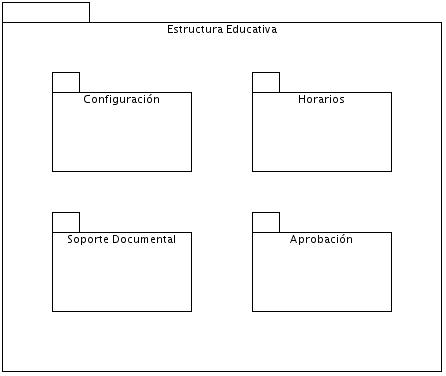
\includegraphics[width=1\textwidth]{dinamico/images/AL_EE.jpg}}
		\caption{Diagrama de arquitectura lógica de la estructura educativa}
		\label{fig:arquitecturaEE}
	\end{center}
\end{figure}

La figura \ref{fig:arquitecturaAL-MHR} muestra la arquitectura lógica del módulo de horarios. En él se encuentran los submódulos de oferta educativa y definición de horarios.

\begin{figure}[htbp]
	\begin{center}
		\fbox{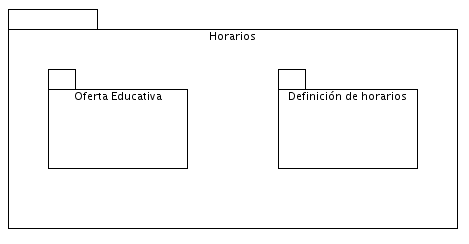
\includegraphics[width=1\textwidth]{dinamico/images/AL-MHR.png}}
		\caption{Diagrama de arquitectura lógica del módulo de horarios}
		\label{fig:arquitecturaAL-MHR}
	\end{center}
\end{figure}

La figura \ref{fig:ofertaEducativa} muestra los casos de uso del submódulo de oferta educativa, mediante los cuales se gestionan las unidades de aprendizaje que se impartirán en el periodo escolar inmediato siguiente, el llenado y monitoreo de las unidades de aprendizaje que solicitan los profesores.

\begin{figure}[htbp]
	\begin{center}
		\fbox{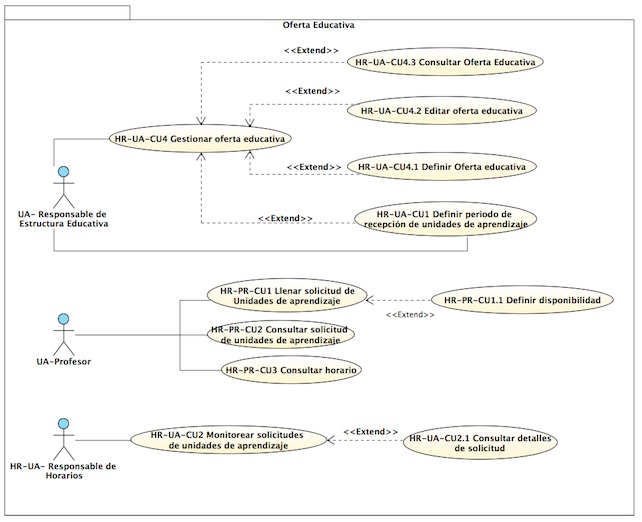
\includegraphics[width=1\textwidth]{dinamico/images/HR_DCU.jpg}}
		\caption{Diagrama de casos de uso del submódulo de oferta educativa}
		\label{fig:ofertaEducativa}
	\end{center}
\end{figure}

La figura \ref{fig:definicionHorarios} muestra los casos de uso del submódulo de definición de horarios, el cuál se divide en la gestión de los grupos y consultas. La gestión de grupos se encarga de las asignaciones de las unidades de aprendizaje, horarios, profesores y espacios.

\begin{figure}[htbp]
	\begin{center}
		\fbox{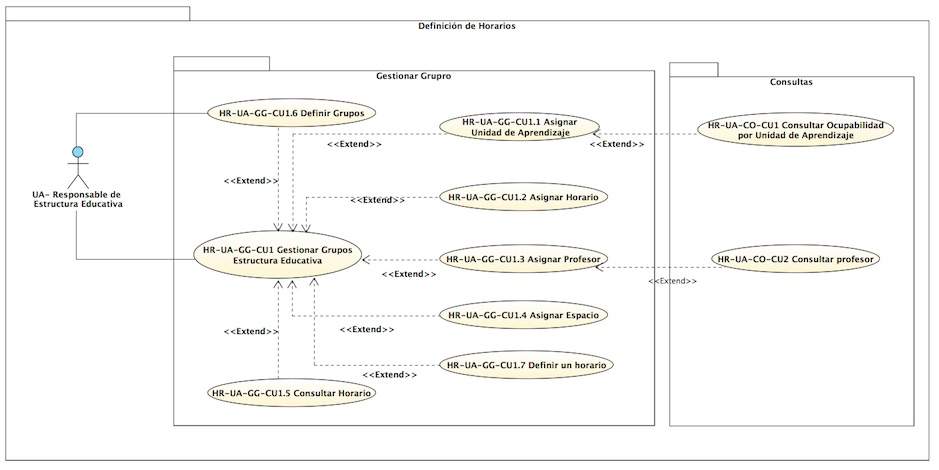
\includegraphics[width=1\textwidth]{dinamico/images/OE_DCU.jpg}}
		\caption{Diagrama de casos de uso del submódulo de definición de horarios}
		\label{fig:definicionHorarios}
	\end{center}
\end{figure}

%La figura \ref{fig:casosDes} muestra los casos de uso para el subsistema DES mediante los cuales se gestionan las unidades de aprendizaje como parte de la gestión de programas académicos.

\begin{figure}[htbp]
	\begin{center}
%		\fbox{\includegraphics[width=1\textwidth]{dinamico/pgpa/images/DES-CUProgramasAcademicos.jpg}}
%		\caption{Diagrama de casos de uso de la gestión de programas académicos}
%		\label{fig:casosDes}
	\end{center}
\end{figure}

%La figura \ref{fig:casosDems} muestra los casos de uso para el subsistema DEMS mediante los cuales se gestionan las unidades de aprendizaje como parte de la gestión de programas académicos.

\begin{figure}[htbp]
	\begin{center}
%		\fbox{\includegraphics[width=1\textwidth]{dinamico/pgpa/images/DEMS-CUProgramasAcademicos.jpg}}
%		\caption{Diagrama de casos de uso de la gestión de programas académicos}
%		\label{fig:casosDems}
	\end{center}
\end{figure}

%La figura \ref{fig:casosUAS} muestra los casos de uso para el subsistema UA del módulo de nivel superior, mediante los cuales gestionan la información de las unidades de aprendizaje.

\begin{figure}[htbp]
	\begin{center}
%		\fbox{\includegraphics[width=1\textwidth]{dinamico/pgpa/images/UAS-CUUnidadesAprendizajeSuperior.jpg}}
%		\caption{Diagrama de arquitectura lógica de la gestión de información de unidades de aprendizaje}
%		\label{fig:casosUAS}
	\end{center}
\end{figure}

%La figura \ref{fig:casosUAMS} muestra los casos de uso para el subsistema UA del módulo de nivel medio superior, mediante los cuales gestionan la información de las unidades de aprendizaje.

\begin{figure}[htbp]
	\begin{center}
%		\fbox{\includegraphics[width=1\textwidth]{dinamico/pgpa/images/UAMS-CUUnidadesAprendizajeMediaSuperior.jpg}}
%		\caption{Diagrama de arquitectura lógica de la gestión de información de unidades de aprendizaje}
%		\label{fig:casosUAMS}
	\end{center}
\end{figure}

